\documentclass[10pt]{report}

\usepackage{makeidx}
\usepackage{mathtools}
\usepackage{amsmath}
\usepackage{amsfonts}
\usepackage{graphicx}
\usepackage{float}

%\usepackage{biblatex}
\title{Dirichlet Mixture in the Extrem}
\author{Samuel Sekarski}
\date{April 2020}
%\makeindex
%\addbibresource{bib.bib}


\begin{document}
\maketitle


%\chapter*{Acknowledgements}

\tableofcontents
%\listoffigures

\chapter{Introduction}
%Motivation, based on chapter 8 (mostly sections 8.1 and 8.2) of Coles (2001) and Boldi and Davison (2007)
%layout of project

Modelling extremes events is becoming more and more important our day and age, mostly in order to asses risks (financial, ecological, structural, ...). Modelling of univariate extremes is well documented and explored, using techniques such as block maximum, threshold and point process.
However, things become, as usual, more complicated in higher dimensions. Multivariate extremes suffer from problems that affect univariate less, such as curse of dimensionality and sparsity.

The most primitive way to deal with multivariate extremes is to study each each component as a univariate process, and then just use univariate techniques. However, this is limiting, as we could easily imaging that there is interdependence of the components amongst themselves, which we lose by considering the components independently. Another reason, as is stated in \cite{Coles}, is that the combination of the individual processes might be of more interest than each process individually.

Analogous methods to block maximum and threshold exist for multivariate cases and we can find models for extremes multivariate events, but we do not have a characterization for the class of all the models. Theorem 8.1 from \cite{Coles} defines a family of bivariate extreme value distributions (and can be generalized to general multivariate case) that arise as the limiting distribution for componentwise block maximas. 

Here is Theorem 8.1 restated (for a bivariate process) for completeness:

Let $M^*_n = (\max_{i=1,...,n} \{X_i\}/n, \max_{i=1,...,n} \{Y_i\}/n)$ be the vector of rescaled componentwise maxima, where $(X_i,Y_i)$ are independent vectors with standard Fréchet marginal distributions. Then if:
$$
Pr\{M^*_n \leq (x,y) \} \xrightarrow[]{d} G(x,y),
$$
where $G$ is a non-degenerate distribution function, $G$ has the form
$$
G(x,y) = 2 \int^1_0 \max (\frac{w}{x},\frac{1-w}{y})dH(w)
$$
and $H$ is a distribution function on $[0,1]$ satisfying the mean constraint
$$
\int_0^1 wdH(w) = 1/2
$$

The problem is that we don't know how to characterize said family ($G$). An approach is to try and approximate the class arbitrarily well, using parametric subfamilies or nonparametric methods and another way is to use nonparametric methods.

Boldi and Davison \cite{BoldiDavison} approached the problem by using a semi-parametric model based on mixtures of Dirichlet distributions that weakly approximate the class of limit distributions.

In this project we will try to use mixes of beta distributions that have been tilted using theorem 2 from Coles and Tawn \cite{ColesTawn} to satisfy the mean constraints.

In section \ref{sec:multivariate} we will discuss how it is possible to tilt a distribution for it to satisfy the mean constraints, how to sample from a tilted distribution, and provide examples of tilted densities and sampling therefrom. 
Next, in section \ref{sec:stats} we will explore how to fit a tilted distribution to some data, using maximum likelihood, fit for some artificially generated data and fit from some real world data, and asses the quality of the fits.

\chapter{Multivariate extremes}
\label{sec:multivariate}
\section{Basic setup}

We will restrict ourselves to the 2 dimensional case but some theorems and results will be stated for arbitrary $D$ dimensions. The $D$-simplex on which our considered distributions will be defined is the set: 
$$
S_D :=\{x \in \mathbb{R}^D | \sum_{i=1}^D x_i = 1\}
$$

In the case $D=2$, that means that we only need to define a distribution on $ x_1 \in [0,1]$ and $x_2$ will simply be $1-x_1$ and therefore $x_2$ is completely determined by $x_1$. As mentioned in the introduction, we are going to consider distributions that are a mix of $K$ beta distributions:

$$
\nu^*(x_1,x_2) = \prod_{k=1}^K \pi_k Beta(x_1;\alpha_k,\beta_k)
$$
with
$$
\prod_{k=1}^K \pi_k= 1
$$

The mean of this distribution is:
$$
\mathbb{E}[X_1] = \sum_{k=1}^K \pi_k\frac{\alpha_k}{\alpha_k + \beta_k}, \hspace{10pt} (X_1,X_2) \sim \nu^*
$$

however this is in general not equal to $1/2$ and so this class of distributions does not satisfy the criteria of Theorem 8.1.
In section \ref{sec:tilting} we will see how to tilt a wide class of distributions to force the mean constraint $1/D$ to hold, and will apply it to our case.

\section{Construction of angular distributions}
\label{sec:tilting}
%using thm 2 of Coles and Tawn (1991)
%What I already have in this section plus simple explanation
%examples of simulation and tilting

The main tool for tilting distributions, is theorem 2 from the 1991 paper from Coles and Tawn \cite{ColesTawn}, which we state again here for completeness:\\

Theorem 2:\\
If $h*$ is any positive function on $S_D$ with finite first moments, then

$$
h(w) = (m*w)^{-(D+1)}D^{-1}\prod_{d=1}^{D}m_dh^*\left(\frac{m_1w_1}{m*w}, \ldots , \frac{m_Dw_D}{m*w}\right)
$$

where

$$
m_d = \int_{S_D} u_dh^*(u)du, \quad d=1, \ldots ,D,
$$

satisfies mean constraints $1/D$ and is therefore the density of a valid measure function $H$.
\\

To verify this that the theorem holds, we to verify that the Jacobian of the transformation:

$$
W_d = \dfrac{W^*_d/m_d}{\sum_{c=1}^{D}W_c^*/m_c},\hspace{10pt}
W_d^* = \frac{m_dW_d}{\sum_{c=1}^{D}m_cW_c},\hspace{10pt}
d=1,...,D.
$$

is in fact $|\partial w^*/\partial w | = (m^Tw)^{-D} \prod_{d=1}^{D}m_d$.
To do this, we rewrite the first transformation as:

$$
w_s^* = \frac{m_dw_d}{m_D+\sum_{c=1}^{D-1}(m_c - m_D)w_c}, \hspace{10pt}
d=1,...,D-1.
$$

by noting that $w=(w_1,...w_D)$ belongs to the D-1 simplex. To simplify notation, we write
$m^Tw = m_D + \sum_{c=1}^{D-1}(m_c - m_D)w_c$. As such,

$$
\partial w_d^*/\partial w_d = m_d/(m^Tw) - m_dw_d(m_d - m_D)/(m^Tw)^2
$$
$$
\partial w_d^*/\partial w_c = - m_dw_d (m_c - m_D)/(m^Tw)^2
$$

This defines a matrix that we can write as $A + ab^T$ where:
$$
A = diag(m_1,...,m_{D-1})/(m^Tw)
$$
$$
a = (m_1w_1,...,m_{D-1}w_{D-1})^T
$$
$$
b = -(m_1 - m_D,...,m_{D-1} - m_D)^T/(m^Tw)^2
$$

Let's recall the determinant lemma:
Let $A$ be an invertible $ p * p $ matrix, and $a,b,$ be vectors of length $p$.
Then $|A + ab^T| = |A|(1 + b^TA^{-1}a)$ \\

In our case, $A$ is a diagonal matrix, so $|A| = (m^Tw)^{-(D-1)} \prod_{c=1}^{D-1}m_c$\\
and $b^TA^{-1}a = -\frac{m^Tw + m_D}{m^Tw}$ so $1 + b^TA^{-1}a = m_D/m^Tw$.

Therefore, $|\partial w^*/\partial w| = (m^Tw)^{-D} \prod_{d=1}^Dm_d$

And thus :

$$
\nu (w) = D^{-1}(m^Tw)^{-(D+1)} (\prod_{d=1}^D m_d) \nu^* (\frac{m_1w_1}{m^Tw},...,\frac{m_Dw_D}{m^Tw})
$$

\begin{figure}[h]
\centering
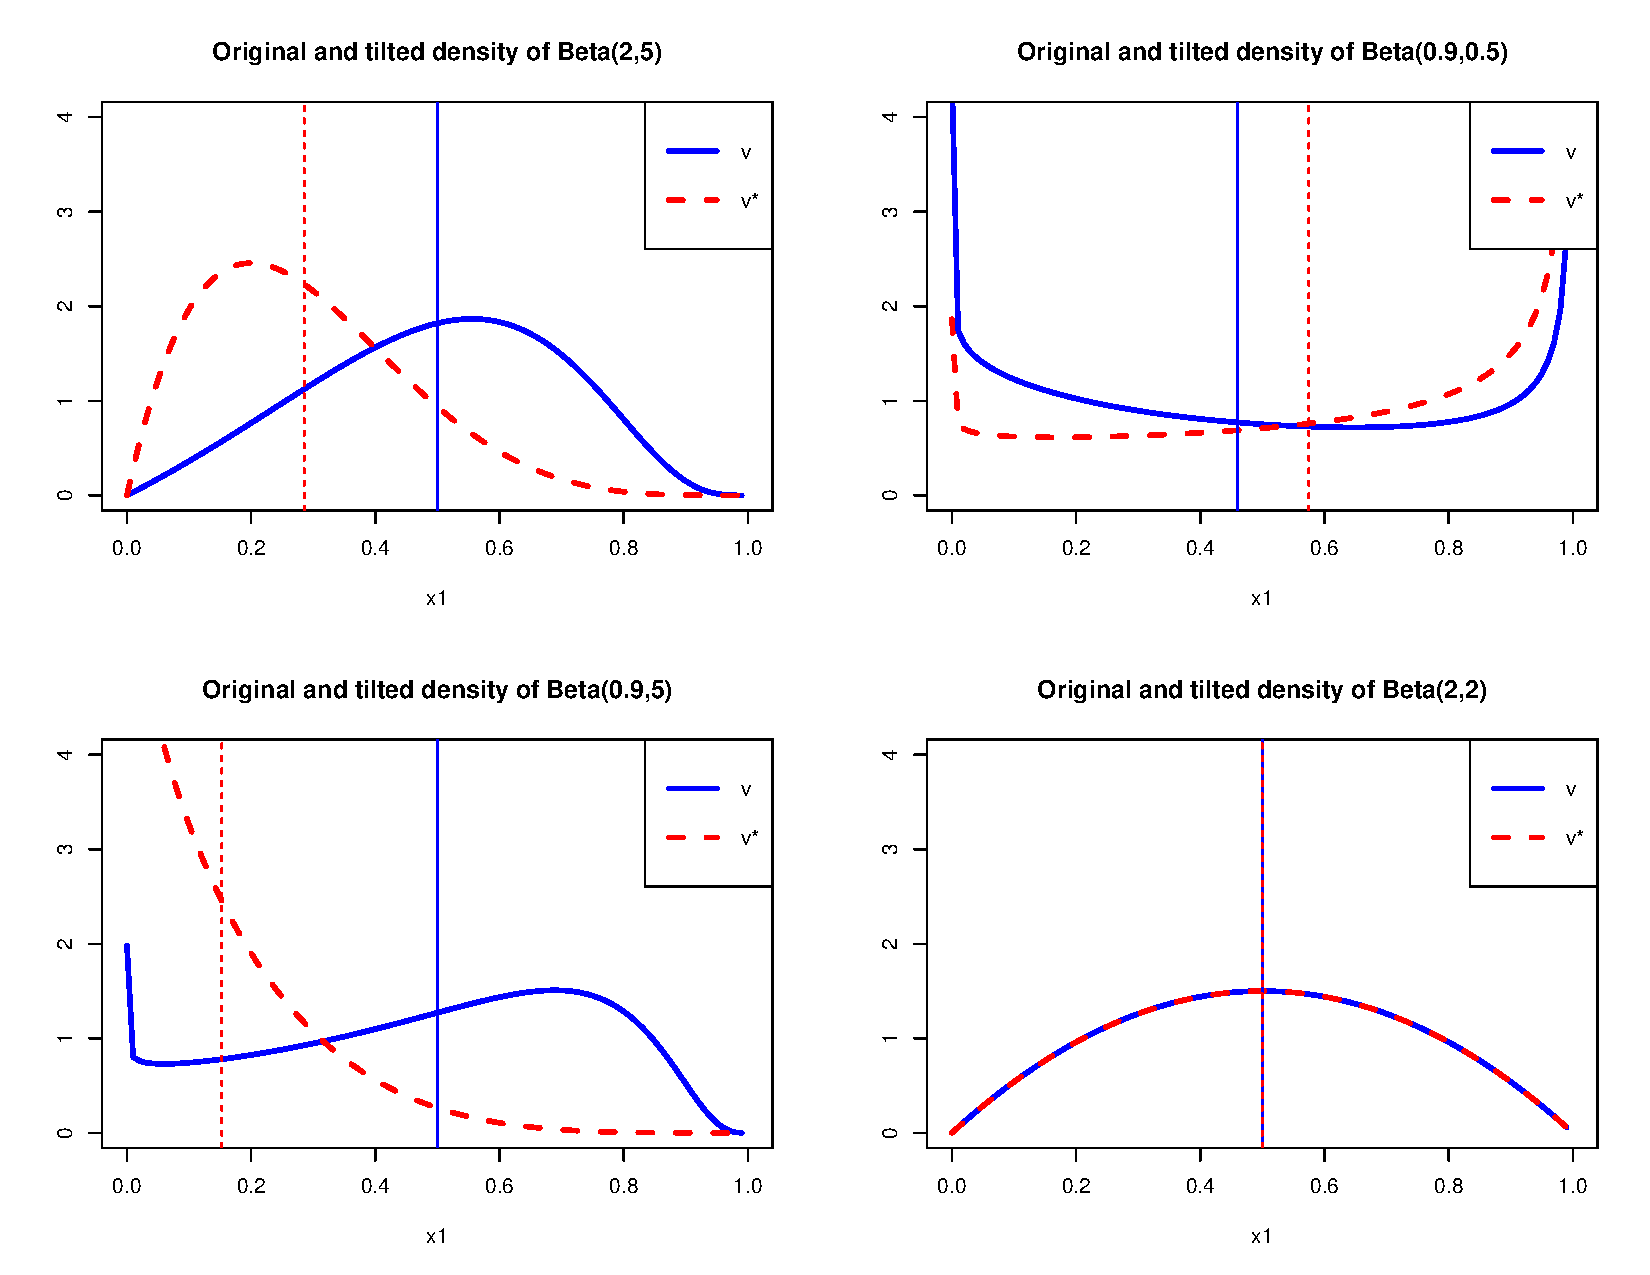
\includegraphics[width=\textwidth]{density_tilt.pdf}
\caption{Graphs of beta distributions for various shape parameters, before and after tilting. The vertical lines represent the mean. As we can see, although the original densities have various means, the tilted densities all have mean 0.5, and when the original distribution already has the correct mean, it is not tilted.}
\label{fig:density_tilt}
\end{figure}

\subsubsection{Sampling from tilted density}
In order to sample from the tilted density, we can sample from the original density, the apply the following Acceptance-Rejection step:

$$
U\leq m_{min}/m^Tw
$$

where $m_{min} = min_d m_d$

The number of accepted samples is proportional to $m_{min}$, so the algorithm is the most efficient when all the $m_d$ are equal

\subsubsection{Tests}
Here are some examples of tilted mixtures of beta distributions, sampled using the algorithm, and the theoretical tilted distributions using the formula.

\begin{figure}[h]
\centering
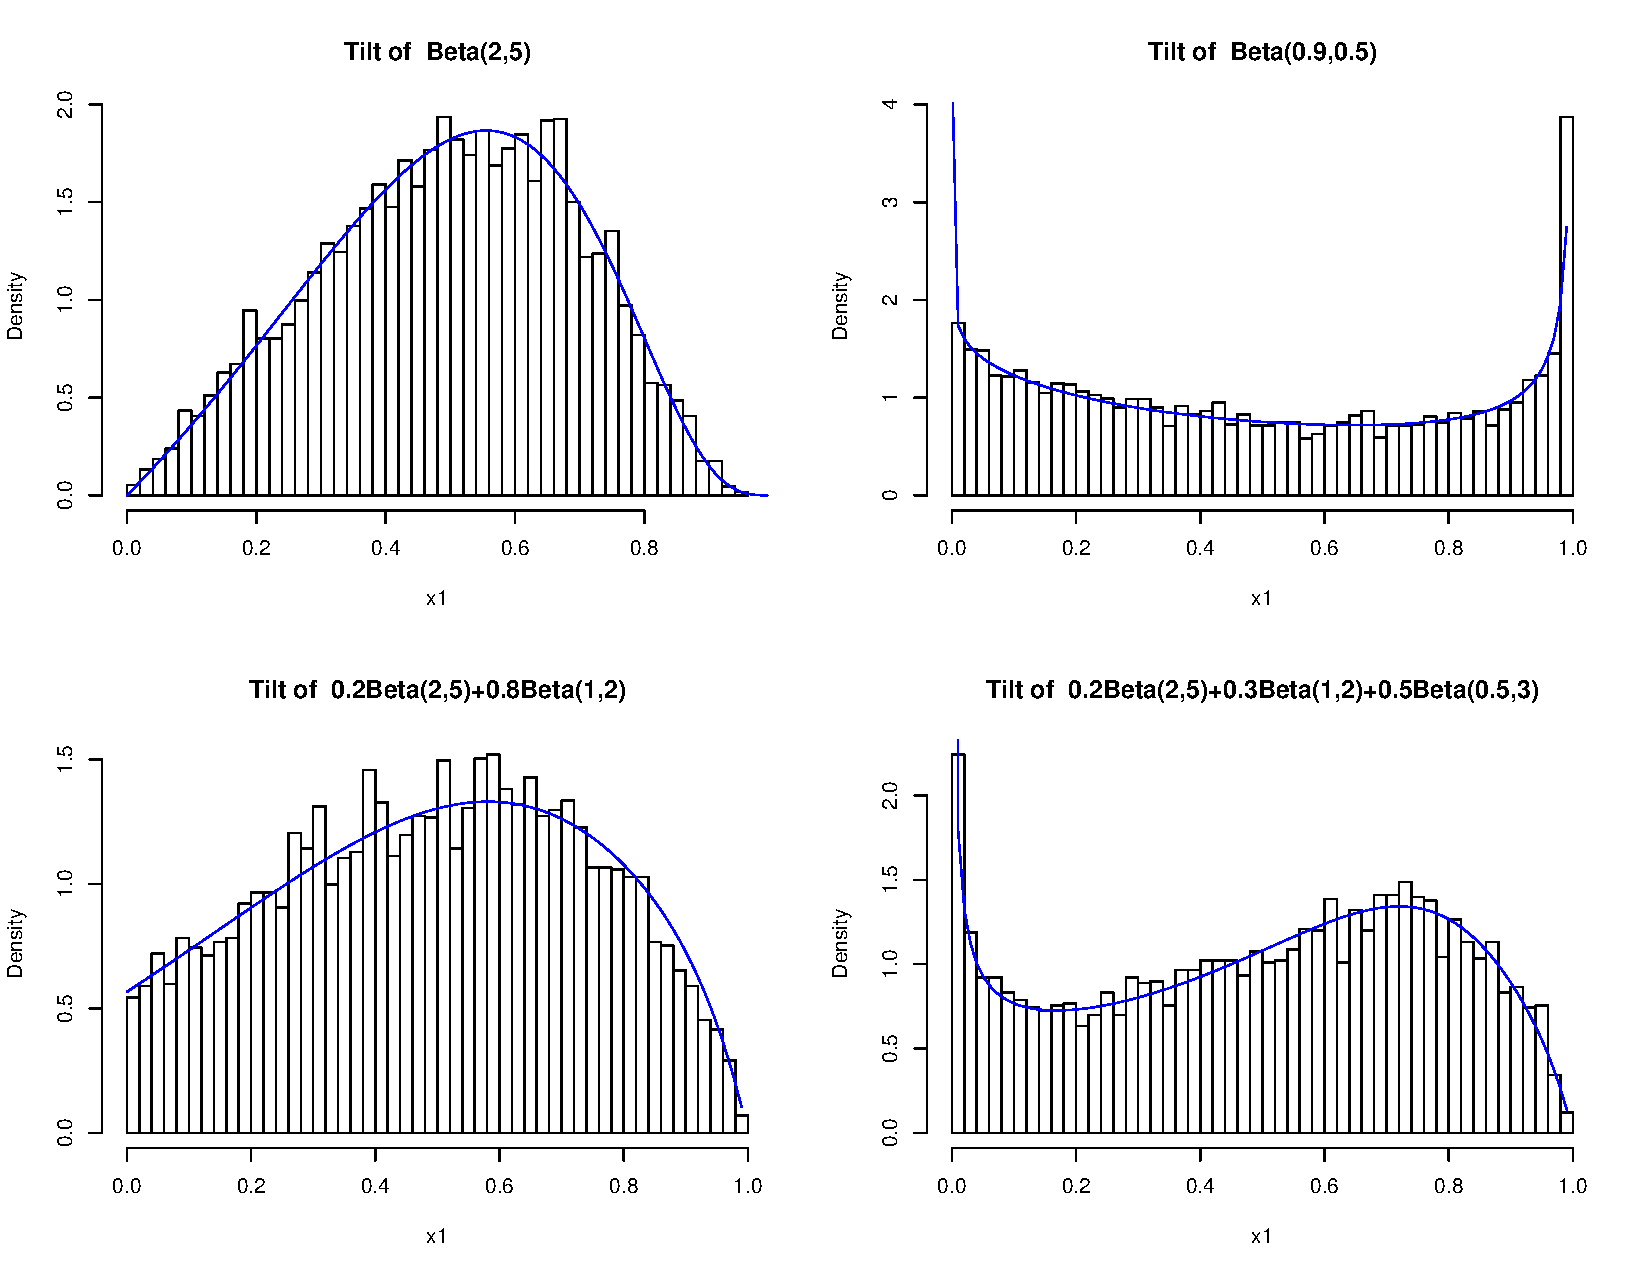
\includegraphics[width=\textwidth]{histogram_tilt.pdf}
\label{fig:historam_tilt}
\caption{Histograms of $10^4$ samples from various mixtures of beta distributions that have been tilted. The pdfs of the distributions are overlayed in blue. As we can see, the sampling algorithm for the tilted mixtures is correctly distributed.}
\end{figure}




\section{Tilted mixtures are dense}
%if possible, show that the class of tilted mixture distributions is dense in the class of distributions with mean 1/D (analogous to Appendix in Boldi and Davison)

\chapter{Statistical aspects}
\label{sec:stats}
\section{Likelihood fitting}
%likelihood fitting of the tilted distribution to data generated from the mixtures
%theory, explanation of how well the ML method works
%use of AIC/BIC to select numbers of components in the fitted mixture

We use the generic R optimiser \textit{optim} for minimise the negative log-likelihood function. In order to use it we first reparameterized the parameters, in order to express the 2-simplex constraint in a way that the optimiser can understand.

$$
\pi_k = \exp(\eta_k)/\left\{ 1+ \sum_{i=2}^K\exp(\eta_i)\right\}, \quad k=2,\ldots, K, 
$$
and 
$$
\pi_1 = 1/\left\{ 1+ \sum_{i=2}^K\exp(\eta_i)\right\}.
$$

We also reparametrize the $\alpha$ and $\beta$ parameters as:

$$
\alpha_k = log(\xi_k), \quad k=1,\ldots,K,
$$
$$
\beta_k = log(\zeta_k), \quad k=1,\ldots,K
$$

\begin{figure}[h]
\begin{tabular}{cccc}

	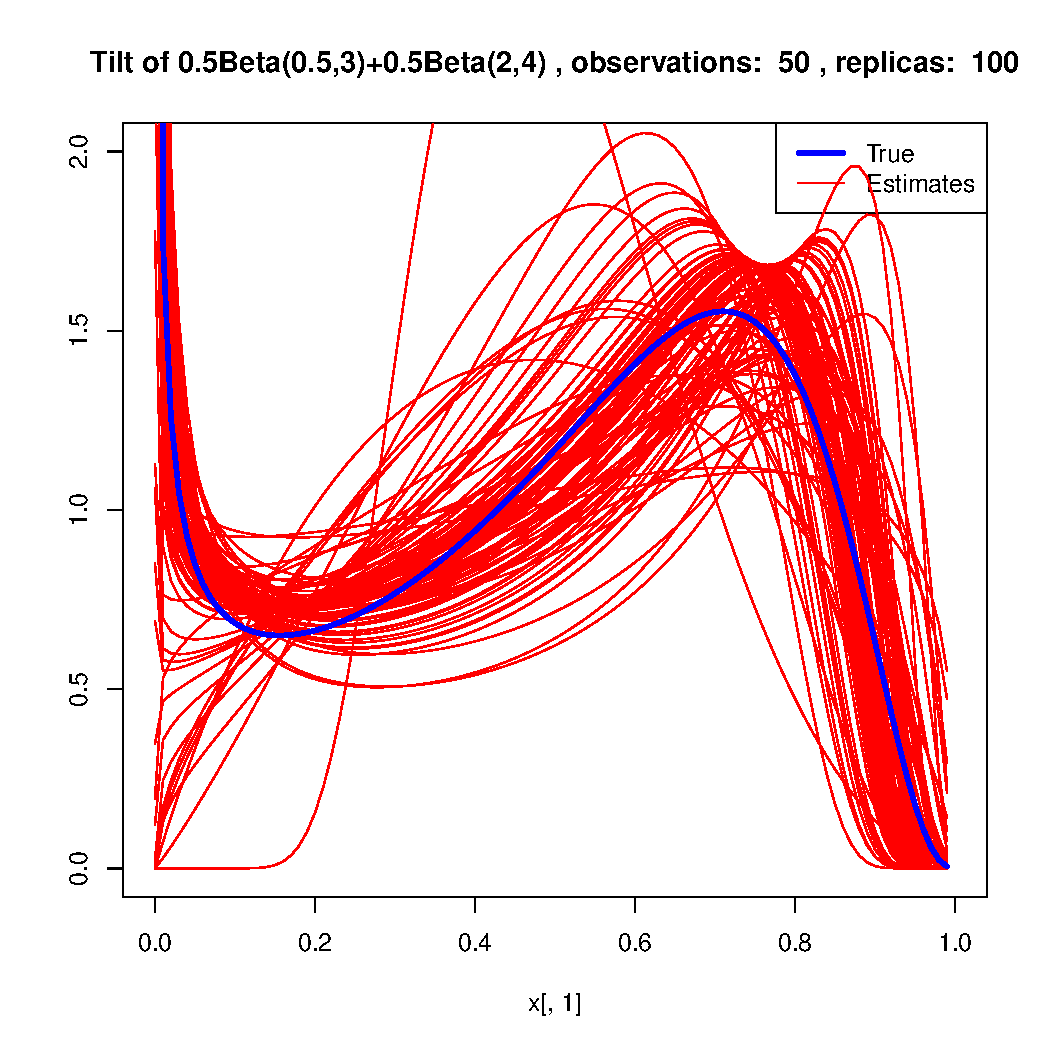
\includegraphics[width=\textwidth/4]{../img/p05_a05_b3_p05_a2_b4/tilted/K1/densities/n50_R100.pdf}
	&
	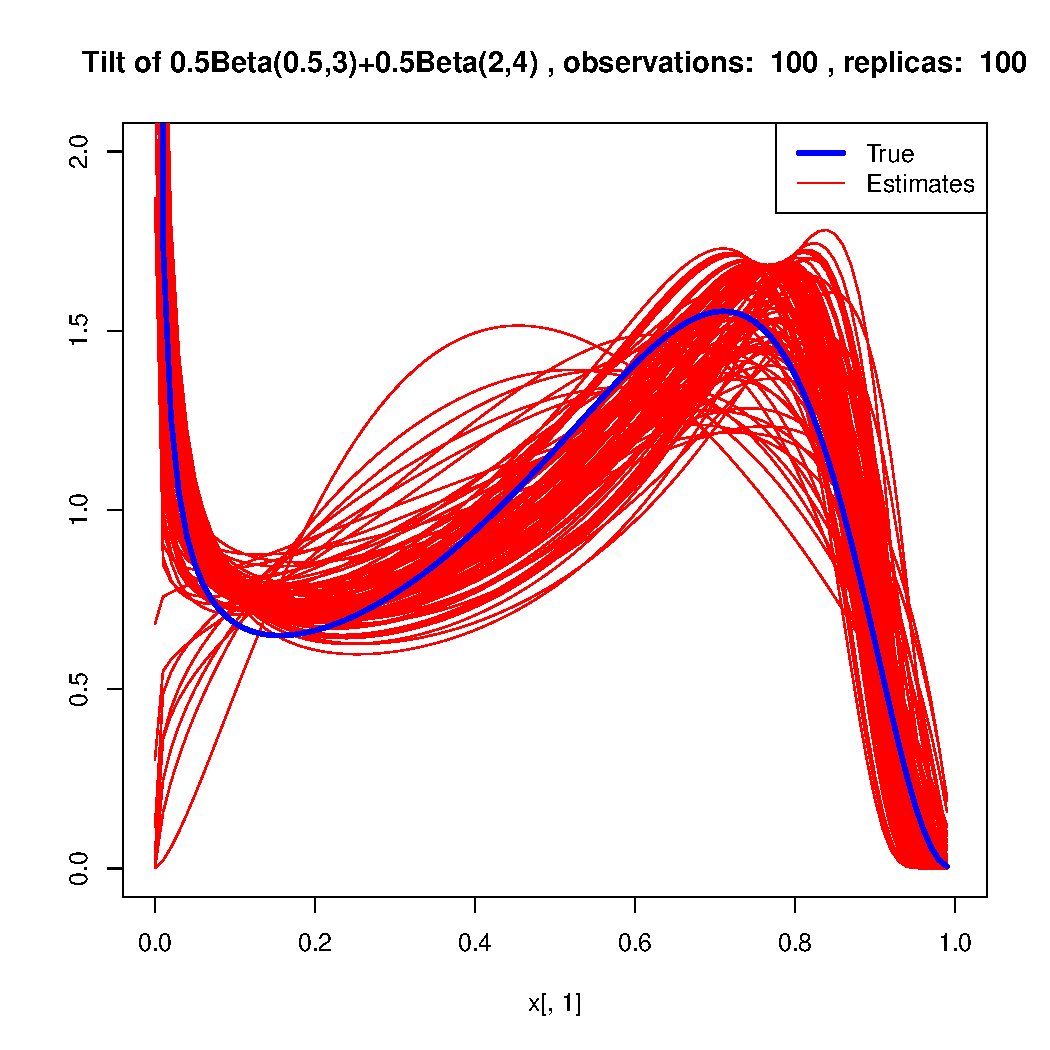
\includegraphics[width=\textwidth/4]{../img/p05_a05_b3_p05_a2_b4/tilted/K1/densities/n100_R100.pdf}
	&
	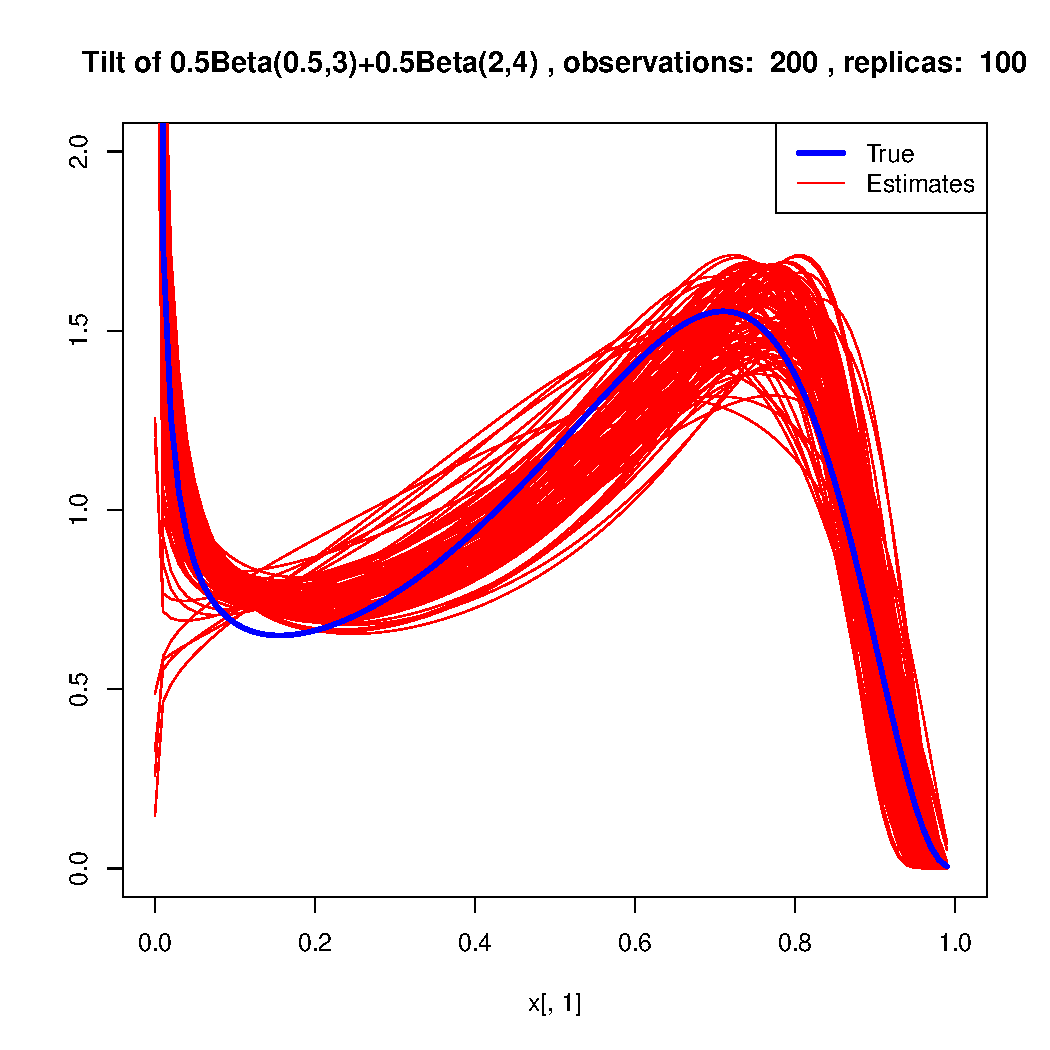
\includegraphics[width=\textwidth/4]{../img/p05_a05_b3_p05_a2_b4/tilted/K1/densities/n200_R100.pdf}
	&
	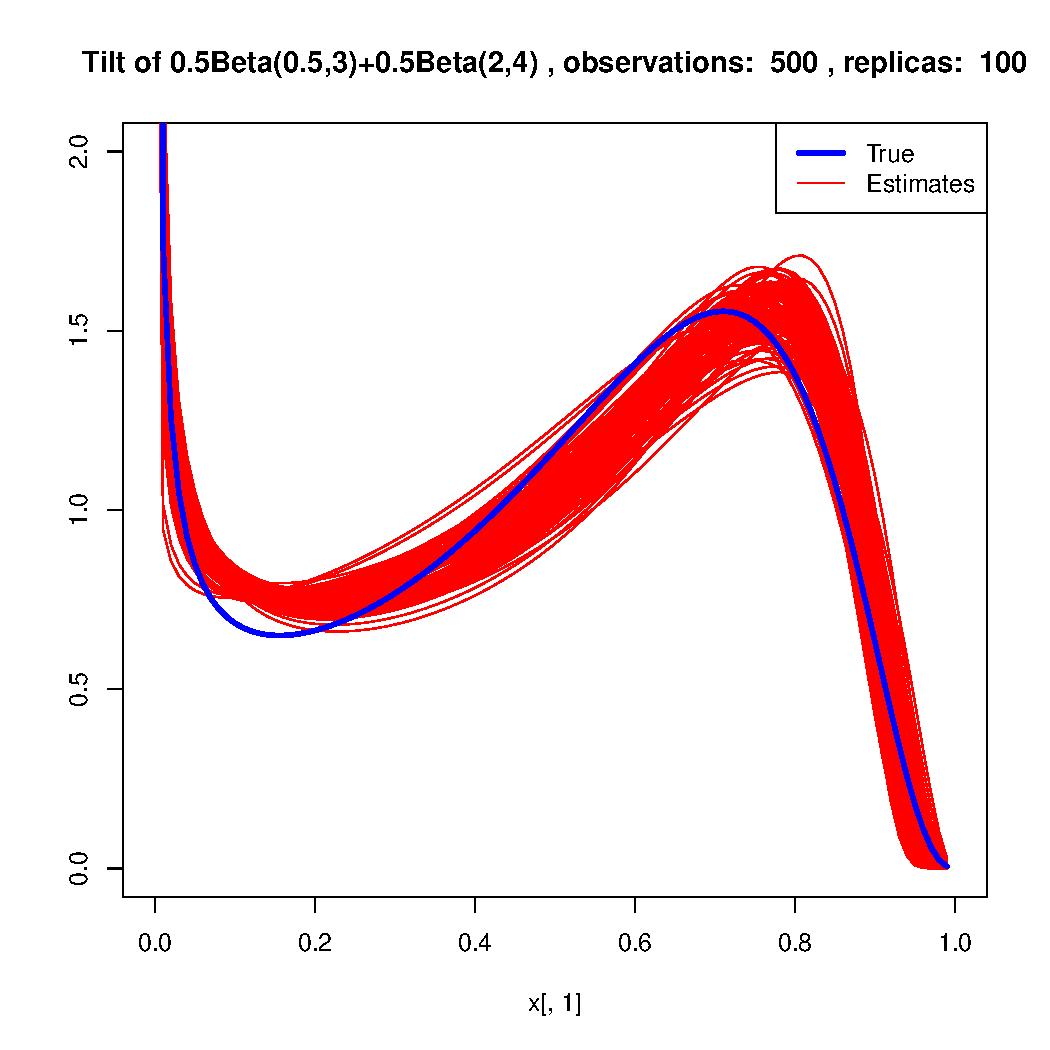
\includegraphics[width=\textwidth/4]{../img/p05_a05_b3_p05_a2_b4/tilted/K1/densities/n500_R100.pdf}\\
	
	
	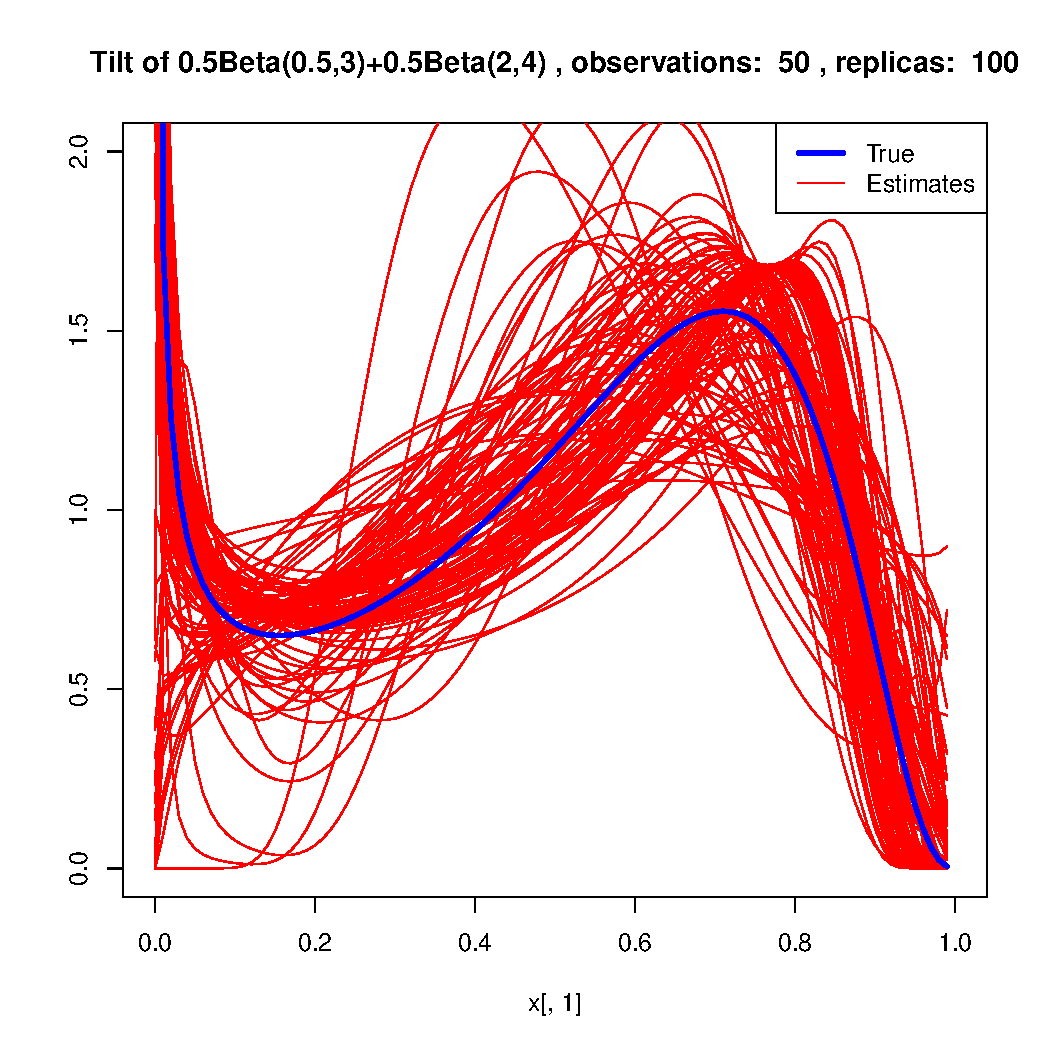
\includegraphics[width=\textwidth/4]{../img/p05_a05_b3_p05_a2_b4/tilted/K2/densities/n50_R100.pdf}
	&
	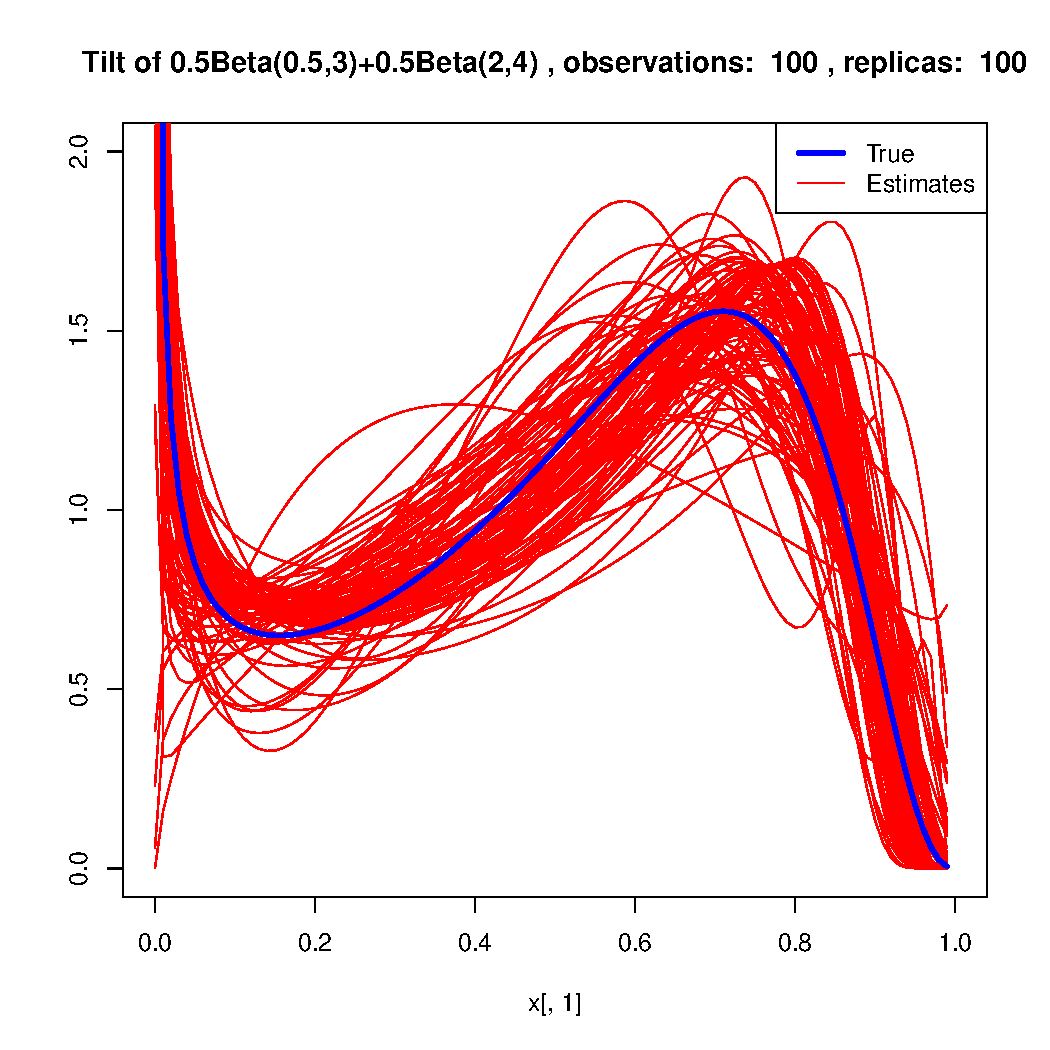
\includegraphics[width=\textwidth/4]{../img/p05_a05_b3_p05_a2_b4/tilted/K2/densities/n100_R100.pdf}
	&
	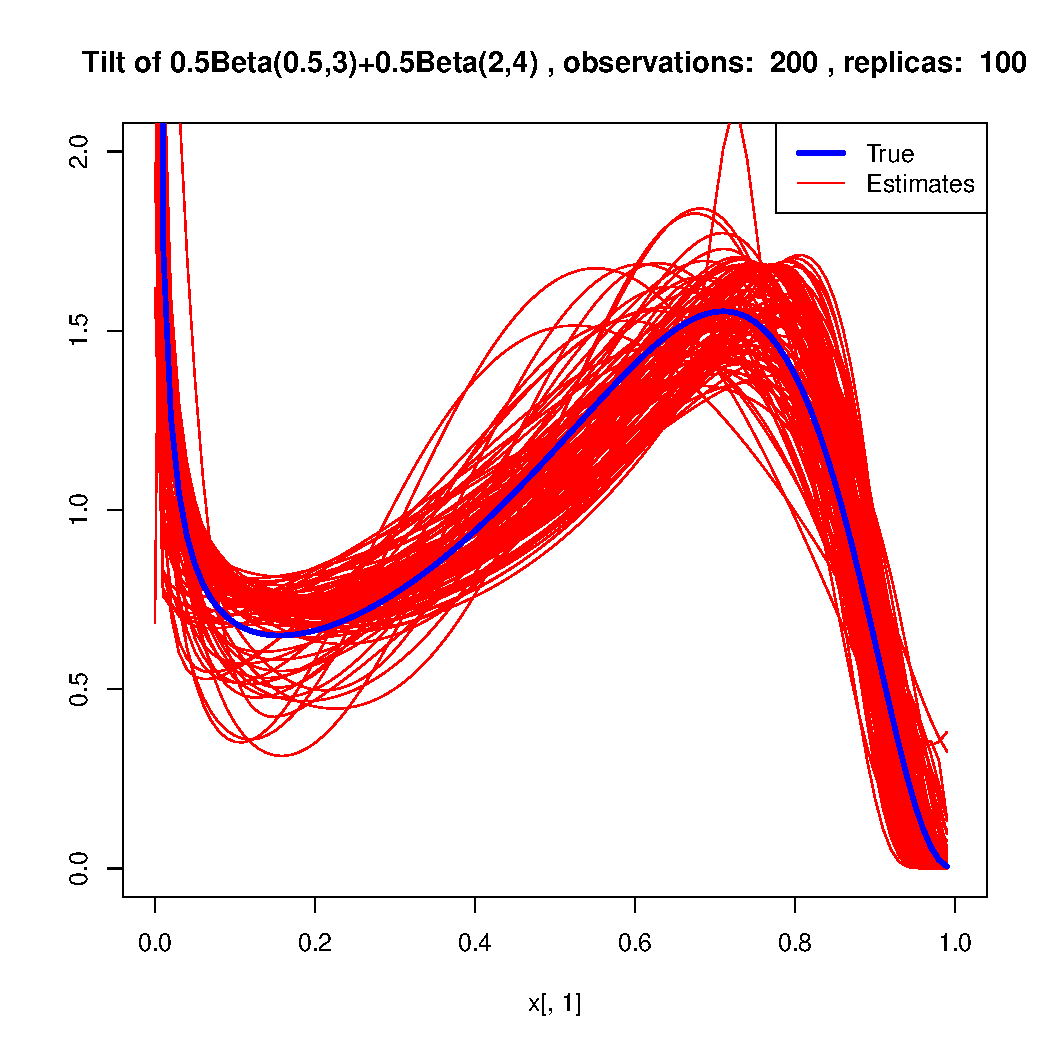
\includegraphics[width=\textwidth/4]{../img/p05_a05_b3_p05_a2_b4/tilted/K2/densities/n200_R100.pdf}
	&
	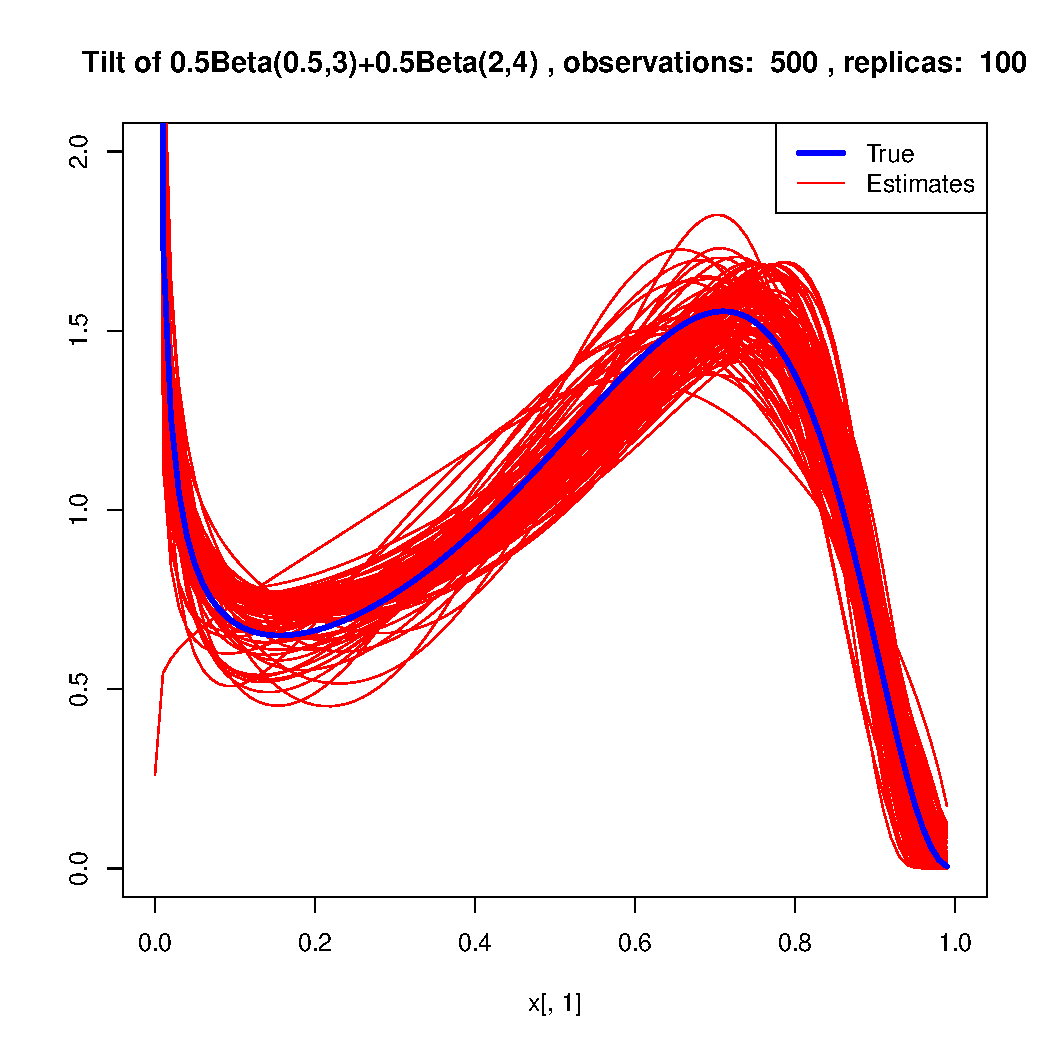
\includegraphics[width=\textwidth/4]{../img/p05_a05_b3_p05_a2_b4/tilted/K2/densities/n500_R100.pdf}\\
	
	
	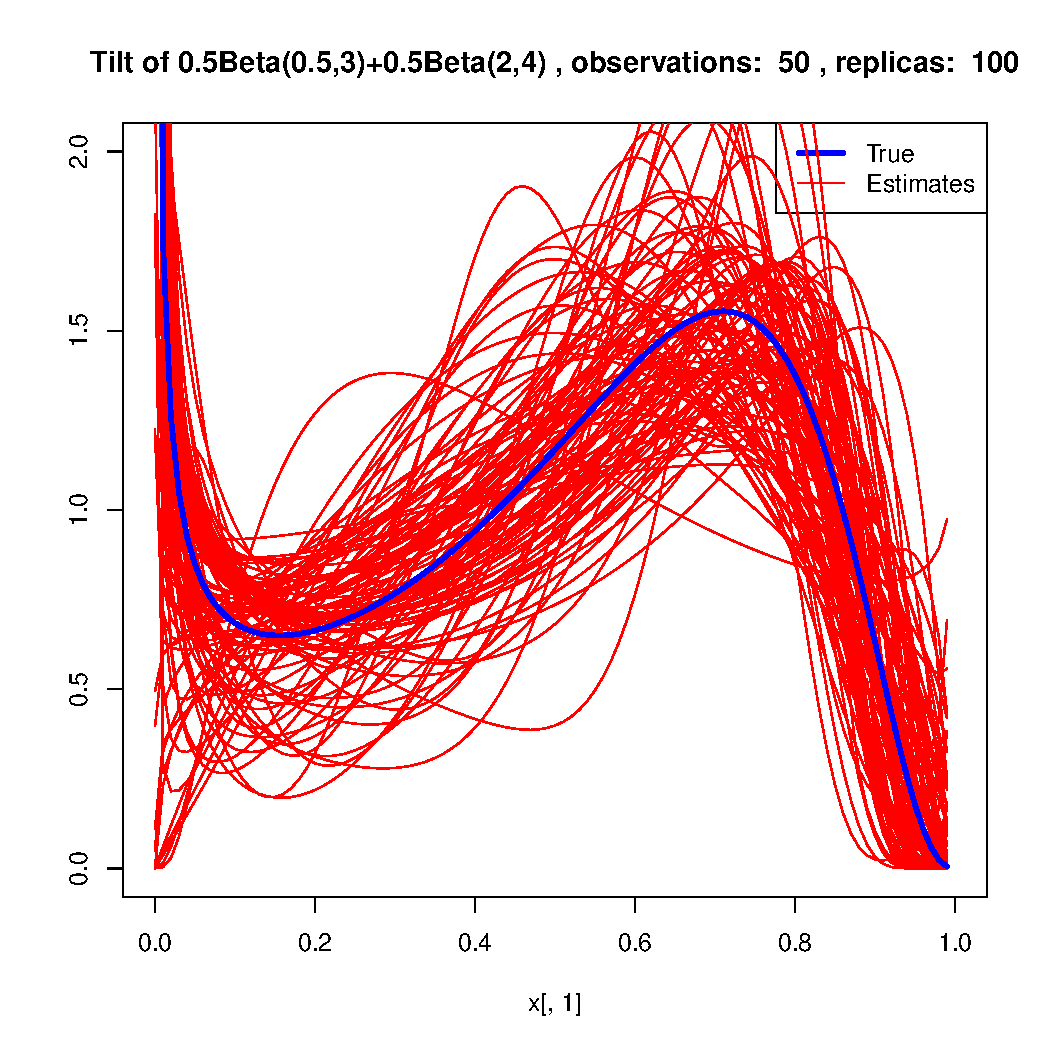
\includegraphics[width=\textwidth/4]{../img/p05_a05_b3_p05_a2_b4/tilted/K3/densities/n50_R100.pdf}
	&
	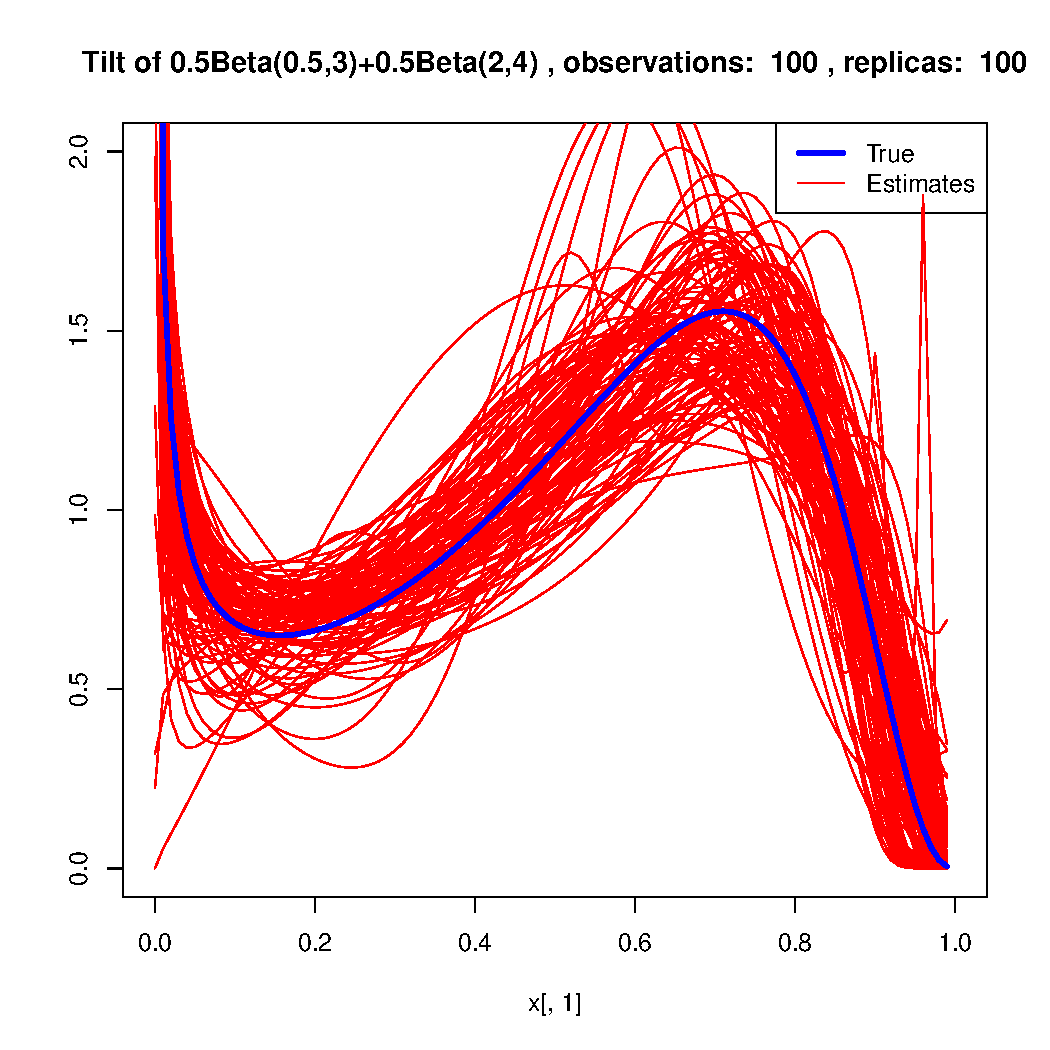
\includegraphics[width=\textwidth/4]{../img/p05_a05_b3_p05_a2_b4/tilted/K3/densities/n100_R100.pdf}
	&
	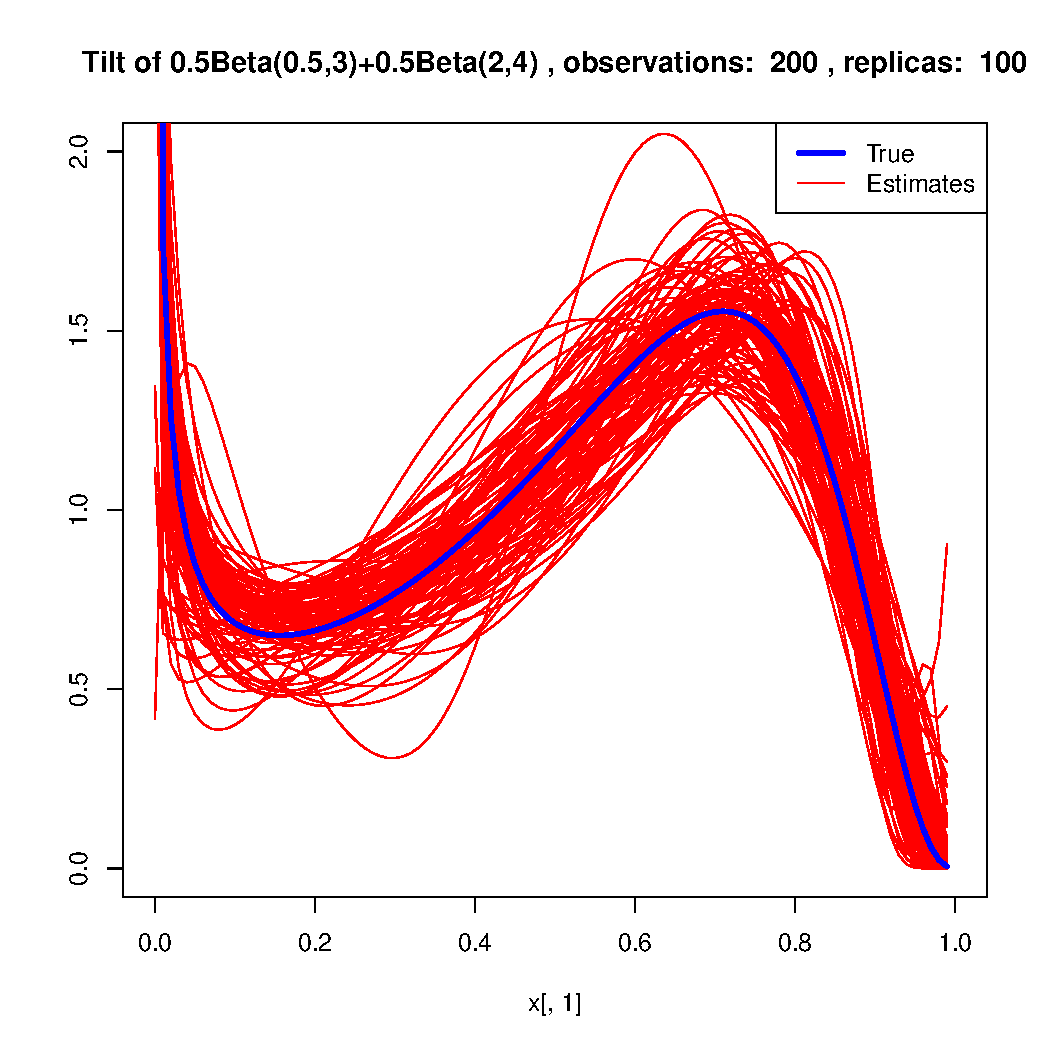
\includegraphics[width=\textwidth/4]{../img/p05_a05_b3_p05_a2_b4/tilted/K3/densities/n200_R100.pdf}
	&
	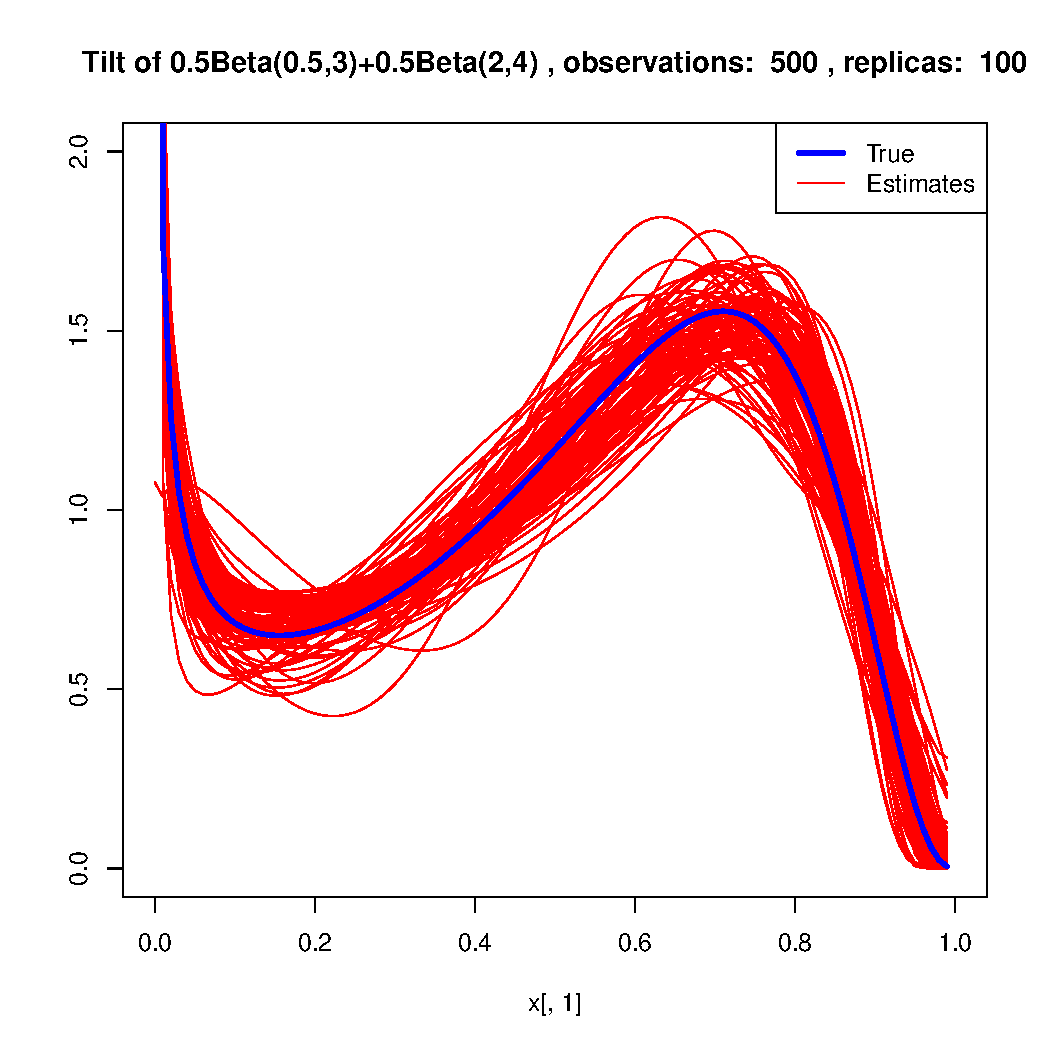
\includegraphics[width=\textwidth/4]{../img/p05_a05_b3_p05_a2_b4/tilted/K3/densities/n500_R100.pdf}\\
	
\end{tabular}
\label{fig:TDB1}
\caption{MLE fits to samples of size, from left to right, $n=50$, $n=100$, $n=200$ and $n=500$, with different number of betas in the mix. From top to bottom: $K=1$, $K=2$ (which is the number that generated the data), and $K=3$, using Nelder-Mead each time, with a maximum of 500 iterations}
\end{figure}

\begin{figure}[h]
\centering
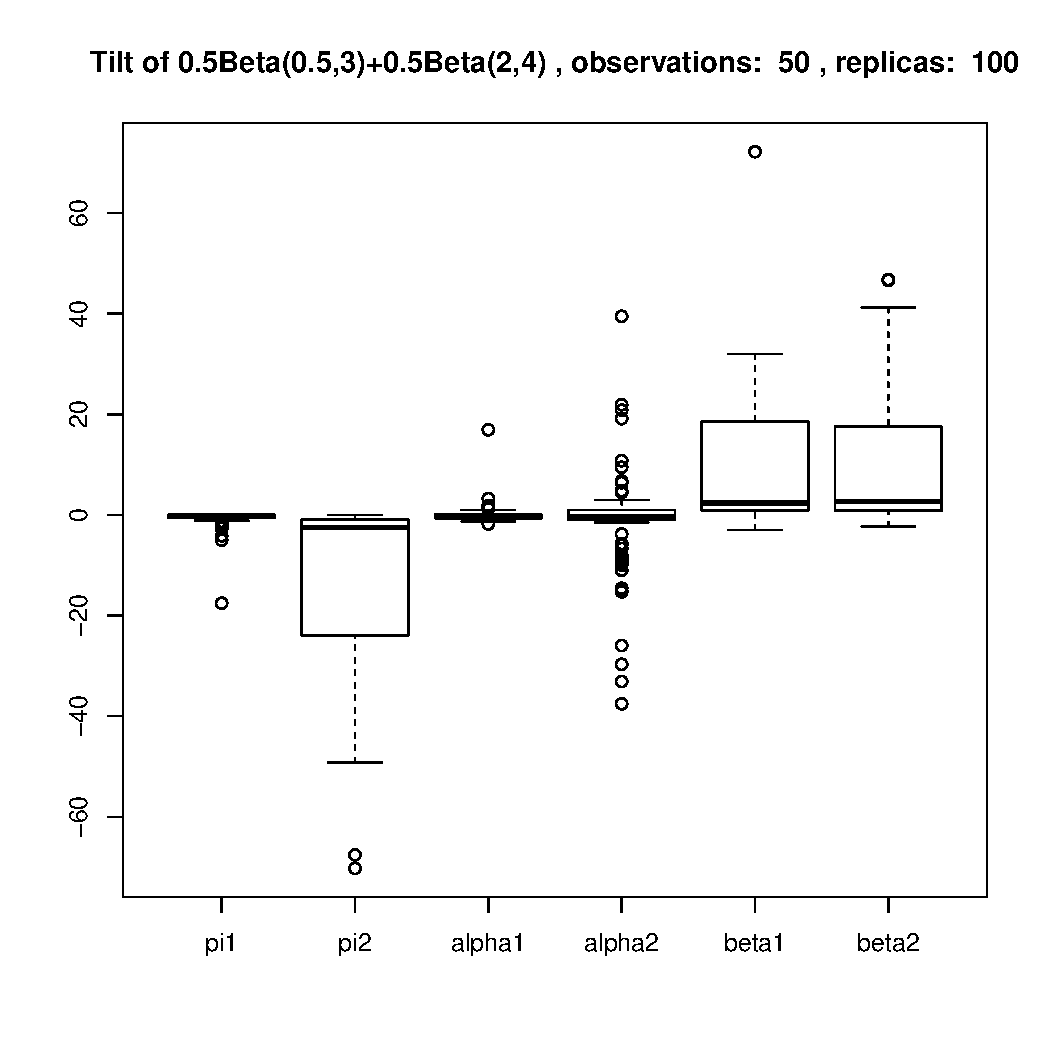
\includegraphics[width=\textwidth]{../img/p05_a05_b3_p05_a2_b4/tilted/K2/bxplots/n50_R100.pdf}
\label{fig:TBD2}
\caption{Boxplot of log MLE estimates (Nelder-Mead, maxit 500), for $K=2$ and sample of 50 observations}
\end{figure}

\begin{figure}[h]
\centering
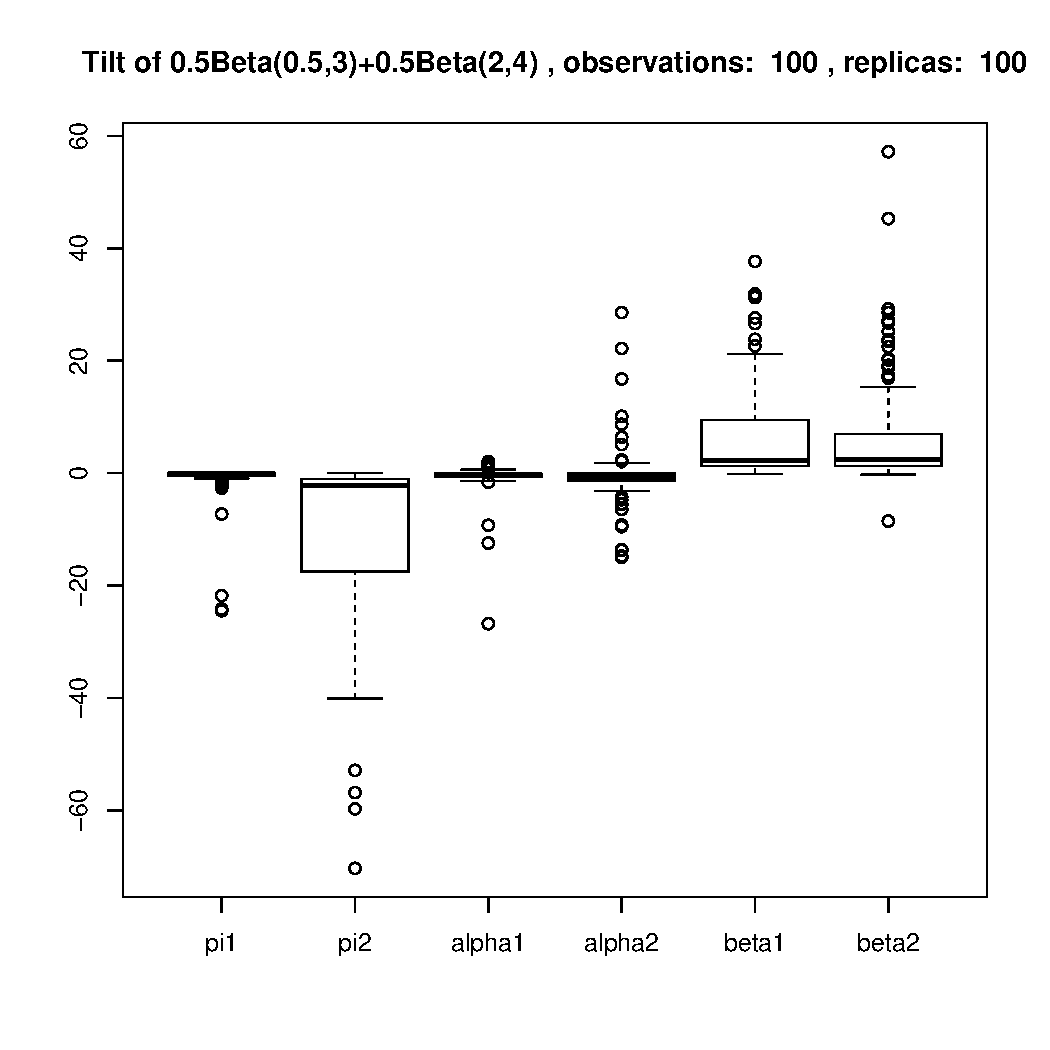
\includegraphics[width=\textwidth]{../img/p05_a05_b3_p05_a2_b4/tilted/K2/bxplots/n100_R100.pdf}
\label{fig:TBD3}
\caption{Boxplot of log MLE estimates (Nelder-Mead, maxit 500), for $K=2$ and sample of 100 observations}
\end{figure}

\begin{figure}[h]
\centering
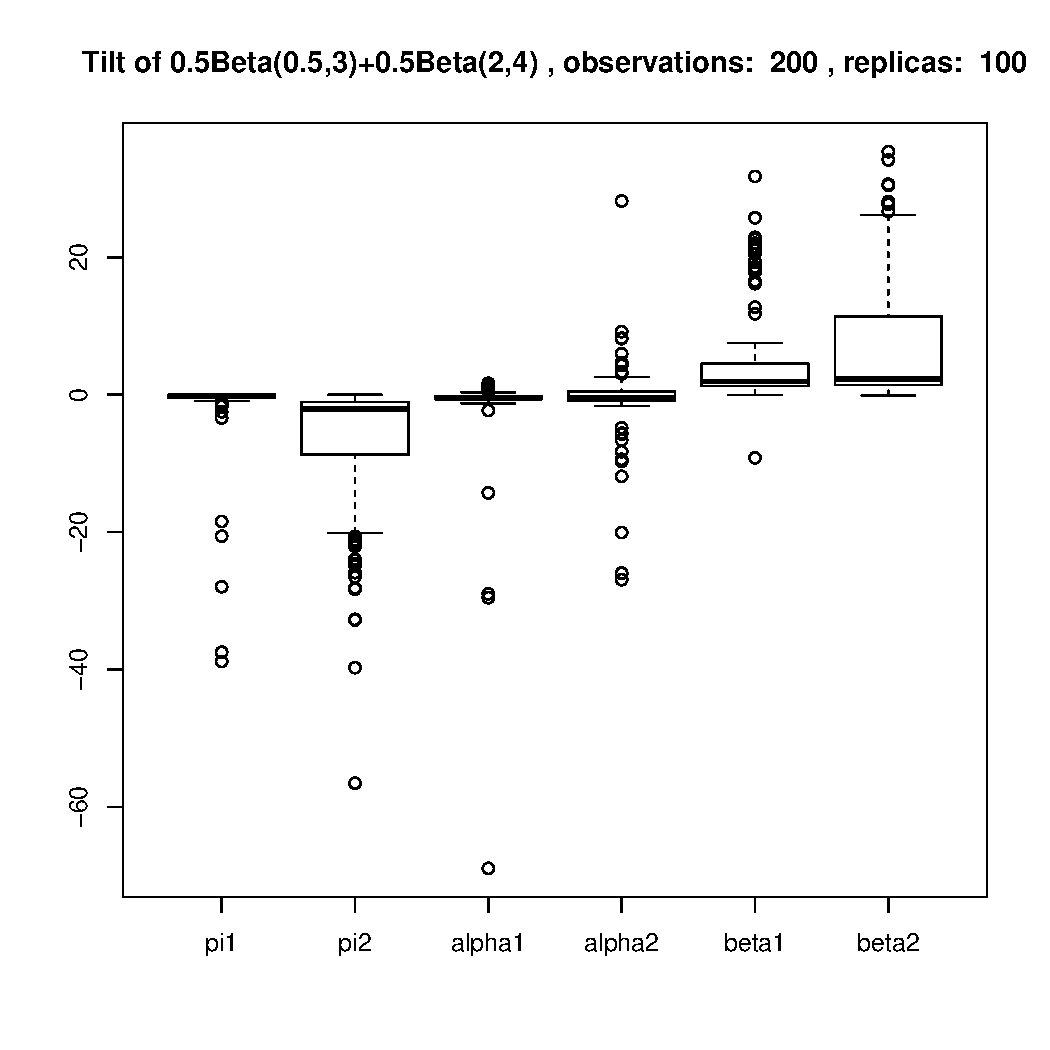
\includegraphics[width=\textwidth]{../img/p05_a05_b3_p05_a2_b4/tilted/K2/bxplots/n200_R100.pdf}
\label{fig:TBD4}
\caption{Boxplot of log MLE estimates (Nelder-Mead, maxit 500), for $K=2$ and sample of 200 observations}
\end{figure}

\begin{figure}[h]
\centering
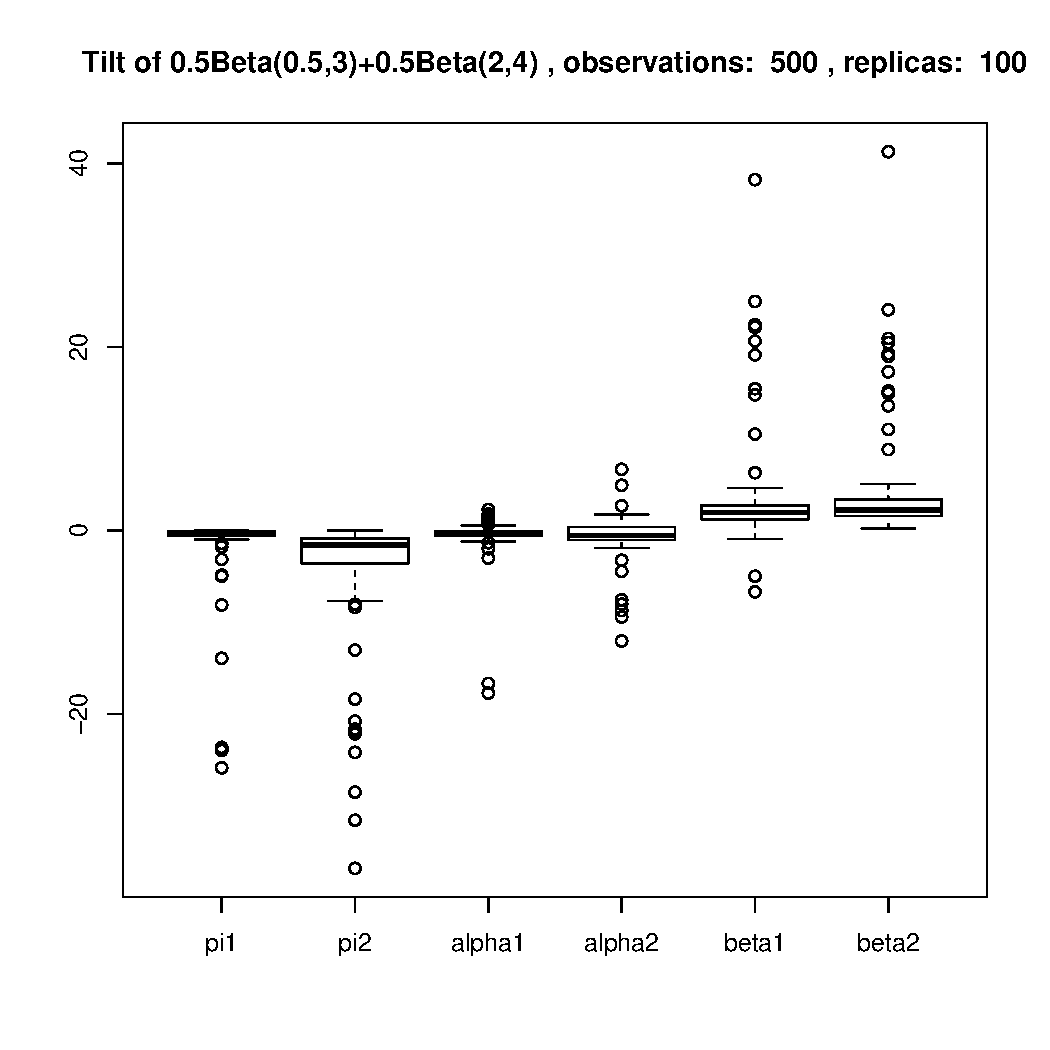
\includegraphics[width=\textwidth]{../img/p05_a05_b3_p05_a2_b4/tilted/K2/bxplots/n500_R100.pdf}
\label{fig:TBD5}
\caption{Boxplot of log MLE estimates (Nelder-Mead, maxit 500), for $K=2$ and sample of 500 observations}
\end{figure}

\begin{figure}[h]
\centering
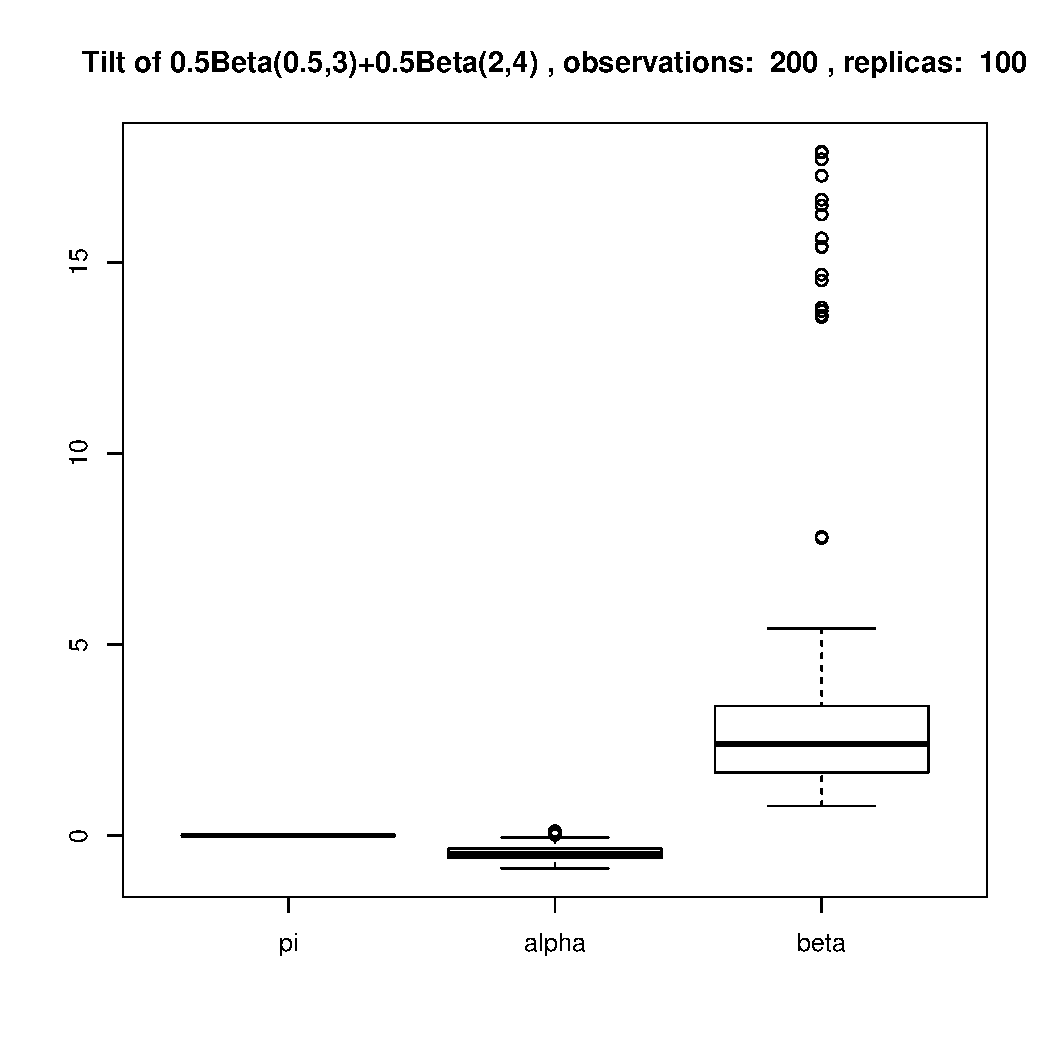
\includegraphics[width=\textwidth]{../img/p05_a05_b3_p05_a2_b4/tilted/K1/bxplots/n200_R100.pdf}
\label{fig:TBD6}
\caption{Boxplot of log MLE estimates (Nelder-Mead, maxit 500), for $K=1$ and sample of 200 observations}
\end{figure}

\begin{figure}[h]
\centering
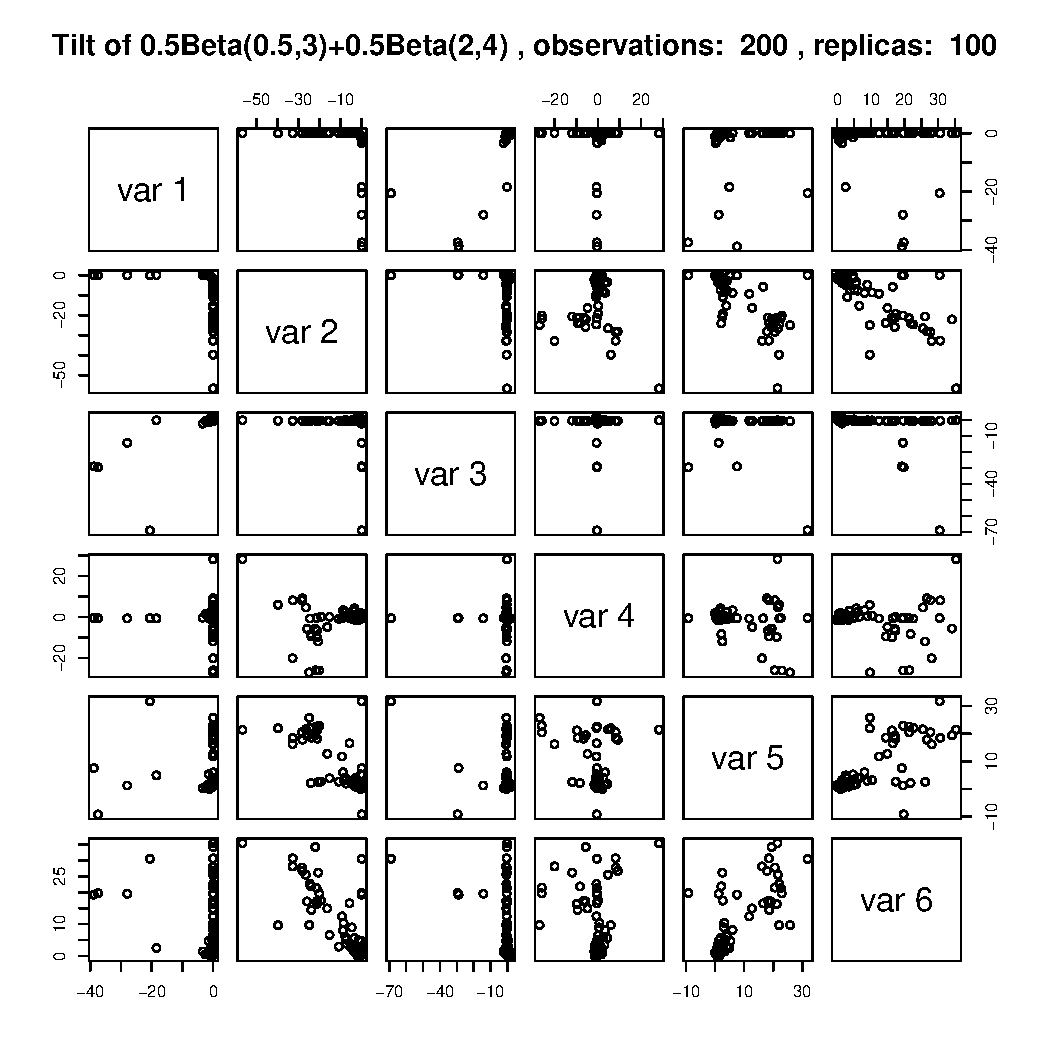
\includegraphics[width=\textwidth]{../img/p05_a05_b3_p05_a2_b4/tilted/K2/pairs/n200_R100.pdf}
\label{fig:TBD7}
\caption{pairs plot of log MLE estimates (Nelder-Mead, maxit 500), for $K=2$ and sample of 200 observations}
\end{figure}

this ensure that the parameters can take any values in $\mathbb{R}$ and there are $3K-1$ parameters to estimate, which can then be transformed back into the original parameterization after estimation. Initially, we consider the K to be a fixed parameter, and for given data we will try to fit with various values of K, including the real value, to see the accuracy, and if values of K that are close, but not correct give a "good enough" estimation (for example we could use a smaller K than the true K and still have a model that is accurate "enough" for certain purposes. The we shall try to consider K as a parameter to be estimated as well, with methods such as step-AIC/BIC to select the model.

\section{Numerical experiments}
%Box plots of estimates and some measure of error (e.g. integrated squared error ? Hellinger distance ?) when (a) true distribution is fitted to the data; (b) data are simulated from some other distribution (i.e. not a mixture)
%for (say) n=50, n=100, n=200, n=500, each with maybe 100, maybe 200 replicates ?



As a measure of the error between the true density $f$ and the estimated density based on n samples $f_n$, we will use the integrated square error, defined as:

$$
err(f_n) := ||f_n - f||^2_2 = \int(f_n(x)-f(x))^2dx
$$

First, in section \ref{sec:truedist} we have fitted a tilted beta mixture to data actually simulated from a tilted beta mixture, then, in section \ref{sec:wrongdist} we have fitted a tilted beta mixture to data simulated from other distributions (i.e. not from a beta mixture).

For each test distribution, we simulate $R=100$ replicas for $n=50$, $n=100$, $n=200$, and $n=500$ observations. The MLE is done with 10 different sets of initial parameters chosen uniformly at random, between $-0.5$ and $+0.5$.

\subsection{Data simulated from mixture}
\label{sec:truedist}

First we generated data using a tilted mix of 2 betas distributions ($0.5Beta(0.5,3) + 0.5Beta(2,4)$) to test how well the maximum likelihood estimation would work. In figure \ref{fig:TDB1} we see that for samples with a high number of observations, even estimating with a different number $K$ of mixes, the results are good, which suggests that we could indeed use a step-AIC/BIC method, starting with a single tilted beta distribution, and keep estimating with more until the added accuracy is no longer significant. Looking at the low observation-size graph, however, we see a lot of volatility and artefacts. Some of the estimations have clearly not converged in 500 iterations of the Nelder-Mead algorithm, even in the case that the correct number $K$ of betas are used.
\\

Looking at the boxplots of the log parameter for the case $K=2$, (figure \ref{fig:TBD2} through \ref{fig:TBD5})we see that there are a lot of very large and very small values. This makes the analysis of the boxplots difficult. But looking at figure \ref{fig:TDB1} we can guess what is happening: as the algorithm fits relatively well with just just a single beta distribution instead of 2, all the cases with a very small $\pi_i$, is just the algorithm fitting one of the component very well, which send the other component to insignificance. As for very small/large value for the $\alpha_i$ and $\beta_i$, our hypothesis is that in the cases where the algorithm fitted one component really well, and the other component can take pretty much any value it wants, as it's contribution to the mix has hardly any weight.
\\

To try to confirm this, first we can look at a boxplot of one of the fits with $K=1$, and indeed if we look at figure \ref{fig:TBD6} we do see that the parameters seem a lot better contained. The group of $\beta$ outliers could be explained by the fact the original density we are working with increases asymptotically on the left side (the side controlled by the $\alpha$ parameters) so the relative importance of the right side (controlled by the $\beta$ parameter) might be low. 
\\

Another check we can do is have a look at a pairs plot for the case $K=2$, to see if low values of $\pi_i$ correlate to very small/large values of $\alpha_i$ and $\beta_i$. In figure \ref{fig:TBD7}, we have the pairs plot for $n=200$ samples. Var2 (a $\pi_i$) vs Var6 (the corresponding $\beta_i$), we clearly see a clump down at the right corner, where stuff is happening according to plan, but also that as the weight of the component gets smaller, the value of the $\beta$ parameter gets larger and more volatile. If we look at Var2 vs Var4 (the corresponding $\alpha_i$), we also see a nice clump around $0$ on the right side, where the weight of the component is still significant, and as the weight gets smaller, the $\alpha$ parameter gets more volatile, with a slight tendency for very small values.
\\


To try and fight this phenomena, we will try 2 things: the first is to used a constrained optimiser (L-BFGS-B) to keep all the log-parameters in a box of say, +/- 20, and the second is to first fit with a single component, and use those estimates, along with added random ones, as a starting point for a round of Nelder-Mead or BFGS (though, considering that the problem seems to be that the algorithms are overfitting one component in neglect of the other, this probably won't help, and method 1 might be the only course of action.)

\subsection{Data simulated from other distributions}
\label{sec:wrongdist}

\section{Numerical experiments}
Much as in the previous section, we have fitted tilted beta mixtures to various simulated data, but this time we also estimate the marginal parameters.

\section{Numerical example}
%Fitting the mixture to some (standard?) datasets to see how many components are needed, asses the quality of the fit, etc.

\chapter{Conclusions}

\begin{thebibliography}{9}

\bibitem{ColesTawn}
S. Coles and A. Twan, \textit{Modelling Extreme Multivariate Events}, Journal of the Royal Statistical Society, 1991

\bibitem{Coles}
S. Coles, \textit{An introduction to statistical modelling of extreme values}, Springer Series in Statistics, 2001


\bibitem{BoldiDavison}
M.-O. Boldi and A. C. Davison, \textit{A mixture model for multivariate extremes}, Journal of the Royal Statistical Society, 2007

\end{thebibliography}


\chapter*{Code}



%\printindex

\end{document}
